\section{BERT}
\label{sec:bert}
At the start of October 2018 Google published their NLP model called Bidirectional Encoder Representations from Transformers (BERT)~\citep{devlin2018}.
The authors show it is able to score state-of-the-art (SOTA) results for eleven NLP tasks.
A comparison by~\citet{young2018recent} shows ELMo~\citep{peters2018} outperforms various SOTA models on six distinct non-trivial NLP tasks.
The comparison~\citep{young2018recent} continues by showing that BERT gets higher accuracy scores than ELMo for all six tasks.
This by transitivity means that BERT obtains the highest accuracy scores at the time of writing.
BERT being SOTA is also supported by a maintained scoreboard for the Stanford Question Answering (SQuAD) dataset~\citep{rajpurkar2019explorer}.

\subsection{Model description}
\label{subsec:model_description}
% empirical results
Results are obtained for a wide range of tasks presented by various datasets.
These tasks include entailment classification, semantic text similarity, sentence classification and question answering.

% technical description
The paper describes three reasons for the good results on the GLUE, MultiNLI and SQuAD datasets.
One being that they pre-train the model and let users fine-tune it on their downstream task~\citep{devlin2018}.
Fine-tuning starts with a model for which all the layers are initialized based upon a pre-trained model~\citep{guo2016deep}.
Then the output layer is replaced by a task specific output layer, hence the number of labels equals the classes in the downstream dataset~\citep{guo2016deep}.
This can also be denoted as transfer learning~\citep{cirecsan2012transfer}.
The output layer uses dropout during training as described in the \textsc{create\_model} function in \textsc{run\_classifier.py}~\citep{devlin2019classifiers}.
Basically, pre-training learns a language model which is used for the downstream task.
Another is that transformer models parallelize better than recurrent architectures~\citep{vaswani2017attention}.
This allowed the BERT researchers to train a model having 340 million parameters (\bert{large}). %bert large
Lastly, the model is presented as being `deeply bidirectional'.
The bidirectionality allows the model to use context from both sides to determine the meaning of a word.
Deep bidirectionality denotes that the model uses left and right context in all layers of the model.
This is visualised and compared to ELMo~\citep{peters2018} and OpenAI GPT~\citep{radford2018improving} in Figure~\ref{fig:bert_comparison}.
\begin{figure}[htbp]
    \begin{center}
        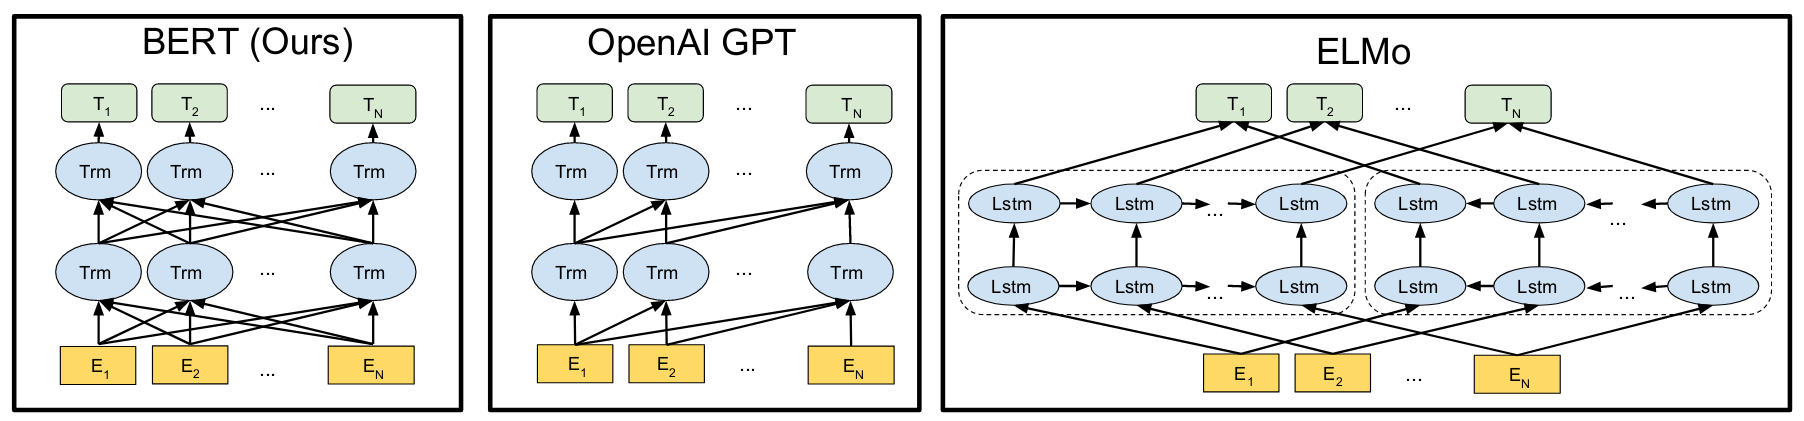
\includegraphics[width=\textwidth]{figures/deeply_bidirectional.png}
    \end{center}
    \caption{
        Comparison of flow of information in the layers of various recent pre-training model architectures~\cite[Figure 1]{devlin2018}.
        Note that ``only BERT representations are jointly conditioned on both left and right context in all layers''~\citep{devlin2018}.
    }
    \label{fig:bert_comparison}
\end{figure}

% available models
Another benefit of BERT is that they provide a wide range of pre-trained models.
The basic models presented in the BERT paper are \bert{base} and \bert{large}.
\bert{base} is ``chosen to have an identical model size as OpenAI GPT for comparison purposes''~\citep{devlin2018}.
\bert{large} obtains higher accuracy on most tasks and has 340 million parameters in total.
Compared to \bert{base} this is an increase from 110 million to 340 million parameters.
The BERT Github repository~\citep{devlin2018github} lists some more models, namely uncased and cased variants for \bert{base} and \bert{large}.
In general uncased models suffice, but for certain tasks (for example, NER) performance can be increased by using a cased model~\citep{devlin2018github}.
Also, they provide \bert{multilingual} and \bert{chinese}.
The multilingual model is trained on the 100 languages having the most Wikipedia pages~\citep{devlin2019multi}.

\subsection{Training}
\label{subsec:training}
% infeasibility of local training
From now on training is used to denote fine-tuning of the model.
Training the general language model on some downstream task is presented as being inexpensive~\citep{devlin2018github}.
Relative to the pre-training it is.
Experiments show that fine-tuning with default hyperparameters will run out of RAM on a 16 GB RAM machine.
Lowering the batch size reduces the memory usage, but running a few training steps still takes at least a few hours.

To train the model on some tasks it is advised to run `a few epochs'~\citep{devlin2018github}.
Based on the example code provided by Google researchers the number of epochs is 3 and the number of training examples is about 1000~\citep{bajaj2018}.
So, it is advised to show the system $3000$ examples.
For our smaller datasets of around 50 examples this means running $3000 / 50 = 60$ epochs.
When measuring the training time in steps it means running $3000 / 16 \approx 188$ steps for a batch size of 16.
Preliminary experiments on the AskUbuntu dataset (having 53 training examples) with a batch size of 32 confirm this estimate, see Figure~\ref{fig:tensorboard}.
The images show that the system does not converge smoothly, and can even have a sudden drop in performance.
One possible explanation for the performance drop is that the model moved into an non-generalizing local minimum.

The results are interesting because it shows that the model is able to learn something even for a dataset with only tens of training examples.
\begin{figure}
    \centering
    \begin{minipage}{0.30\textwidth}
        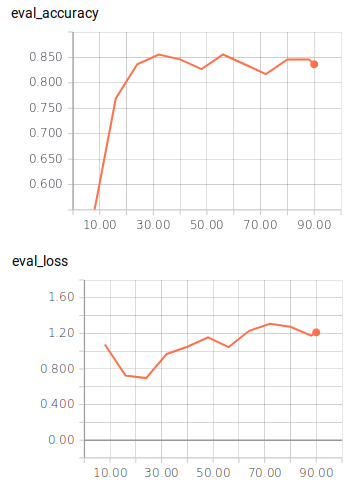
\includegraphics[width=0.9\textwidth]{figures/tensorboard_askubuntu.png}
        \caption*{\bert{base}}
    \end{minipage}
    \hspace*{3mm}
    \begin{minipage}{0.30\textwidth}
        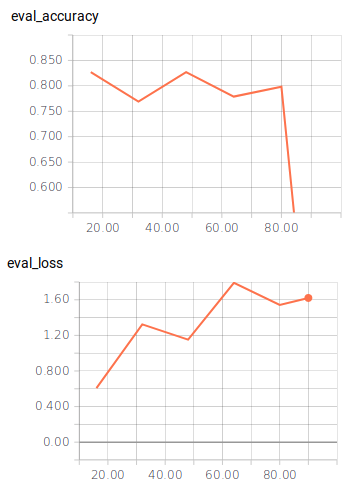
\includegraphics[width=0.9\textwidth]{figures/tensorboard_askubuntu_large.png}
        \caption*{\bert{large}}
    \end{minipage}
    \hspace*{3mm}
    \begin{minipage}{0.30\textwidth}
        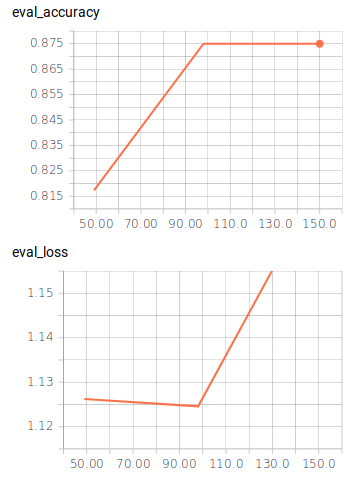
\includegraphics[width=0.9\textwidth]{figures/tensorboard_askubuntu_large_2.png}
        \caption*{\bert{large}, second run}
    \end{minipage}
    \caption{TensorBoard visualisation or `summaries' for fine-tuning pre-trained models on AskUbuntu.
    Here the horizontal axis denotes the number of steps.
    Accuracy and loss for the model trained on the test set is evaluated at fixed steps on the evaluation set.
    The plots show that BERT is in some cases able to converge to a correct local minimum after 100 steps (3200 examples shown to model).
    The scores in these images should not be compared to the scores in Section~\ref{sec:benchmark_results} since the metrics and the data split differ.}
    \label{fig:tensorboard}
\end{figure}
Training the model for 5 steps or 80 examples takes at least a few hours on a modern computer.
Interpolation suggests that training 188 steps will take at least 36 hours.
This is impractical when doing experiments.

% colab intro
According to the paper the benefit of the Transformer models is that they are highly parallelizable.
Training BERT consist mainly of matrix multiplications~\citep{dettmers2018}.
These can be done quickly and efficiently on graphic processing units (GPUs) and tensor processing units (TPUs).
The latter are ASICs created by Google specifically to do machine learning inference~\citep{jouppi2017} and contain 64 GB of RAM~\citep{devlin2018github}.
When using the TensorFlow implementation of BERT GPUs with 16 GB of RAM are required~\citep{devlin2018github}.
GPU optimizations are available in the PyTorch implementation provided by~\citet{wolf2018}, but PyTorch does not support TPUs at the time of writing.
Prices for these GPUs are at least a few thousand euros, which means most users and companies resort to cloud services.
Google Colab~\citet{google2019colab} provides free access to a GPU and TPU instance.
Code which uses Google Colab for BERT is based on an example implementation provided by Google~\citep{bajaj2018}.

% colab usage
Using Colab is a compromise between usability and costs.
The costs are limited to the use of some storage in a Google Cloud Bucket.
Usability is hindered by the usual constraints of online Jupyter Notebook editors, for example no unittests, no autocomplete and poor Git integration.
To overcome these issues most of the code is written and tested locally and pushed to a Github repository called \textsc{improv}, see Appendix~\ref{ch:improv}.
In the Colab the code is then pulled from the repository and main functions are called.
Using Colab has benefits as well.
Hyperparameters and output are visible and can easily be modified in the Notebook, this eases verification.
Reproducibility is possible by opening the Notebook and running all cells.
The first cell will ask to link the Colab to a Google account, make sure this account has access to a Google Cloud Bucket.

% from now on some constraints
The plots in Figure~\ref{fig:tensorboard} are created using the default TensorFlow visualisation tool TensorBoard.
Generating these plots can be done by specifying a model and metrics using the TensorFlow Estimator API.
The plots will not be generated for the rest of the runs for reasons explained in Section~\ref{sec:tpu_and_api}.
For the rest of this document all results are for the \bert{large} model since \bert{base} is only created for a fair comparison with OpenAI GPT~\citep{devlin2018}.

\subsection{Joint training}
\label{subsec:joint_training}
% introduction
One reason why neural networks are obtaining the best results for many fields is because networks are now deep.
Deep networks have more layers and can therefore learn more complex tasks.
One application of this is adding a larger portion of the pipeline to the model.
For example, the code by~\citet{rasa2018config} for the default pipeline for \textsc{rasa-spacy}, as introduced in Section~\ref{subsec:rasa}, contains the following steps.
In these steps a featurizer denotes a system component which transforms text to vector representations~\citep{brutlag2000challenges}.
\begin{enumerate}
    \item Tokenization which splits texts up in tokens.
    \item Regular expression based intent and entity featurizer (for example able to featurize phone numbers),
    \item Intent featurizer based on spaCy~\citep{spacy2019}.
    \item Stanford Named Entity Recognizer based on conditional random fields~\citep{finkel2005incorporating}.
    \item NER synonym detection.
    \item Intent classification based on scikit-learn~\citep{scikit2019}.
\end{enumerate}

For this pipeline the Stanford Named Entity Recognizer and scikit-learn classify separately.
Preferably one would have one model which could learn to do the entire pipeline, also known as an end-to-end model.
End-to-end models have two benefits.
Firstly, an end-to-end model avoids feature engineering and data pre-processing~\citep{ma2016end}.
Secondly, end-to-end models can obtain higher accuracies because (semi-)optimal features are found automatically.

% why it helps
That the combination improves independent models has been shown by~\citet{ma2017jointly} and~\citet{zhang2018joint}.
The results for the former are obtained by using a LSTM network.
The latter introduces an algorithm to combine hidden states from an LSTM.
They show this for the more general problem of sequential labeling and classification.
Intuitively the improvement was to be expected for the following reason.
Suppose we are trying to classify a dataset which contains the sentence:

\begin{center}
    ``I would like to book a ticket to London tomorrow.''
\end{center}

The sentence has intent `BookFlight'.
Training the model could be simplified by providing the sentence classifier with:

\begin{center}
    ``I would like to book a ticket to $<$location$>$ $<$date$>$.''
\end{center}

Now the model does not have to learn to classify sentences while also learning that London is a location and that tomorrow is a date.

% how it should not be done
Note that an end-to-end model is preferred over two separate models.
At the time of writing NER classifiers do not obtain perfect accuracy.
This means that some classifications will be incorrect.
The example from above could instead be converted to:

\begin{center}
    ``I would like to book a $<$date$>$ to $<$location$>$ tomorrow.''
\end{center}

This could make the intent classifier drop in accuracy.
In an ideal end-to-end model incorrect NER classifications would be less of an issue.
The model would learn to ignore the named entity recognition if it would not increase accuracy.

\subsection{BERT joint training}
\label{subsec:bert_joint_training}
% why possible
That joint training BERT is possible can be observed from Figure~\ref{fig:bert_classification}.

\begin{figure}
    \centering
    \begin{minipage}{0.48\textwidth}
        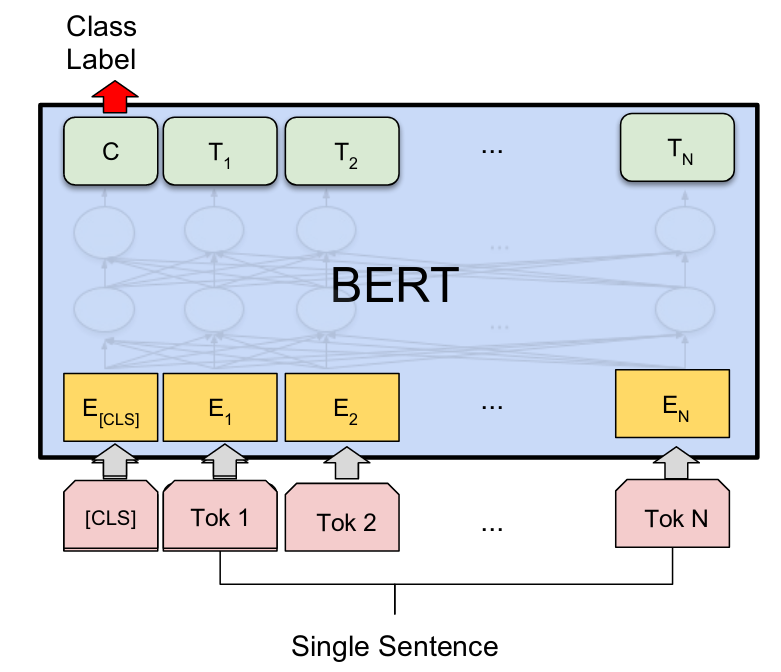
\includegraphics[width=\textwidth]{figures/bert_single_sentence.png}
        \caption*{Single sentence classification}
    \end{minipage}
    \hspace*{3mm}
    \begin{minipage}{0.48\textwidth}
        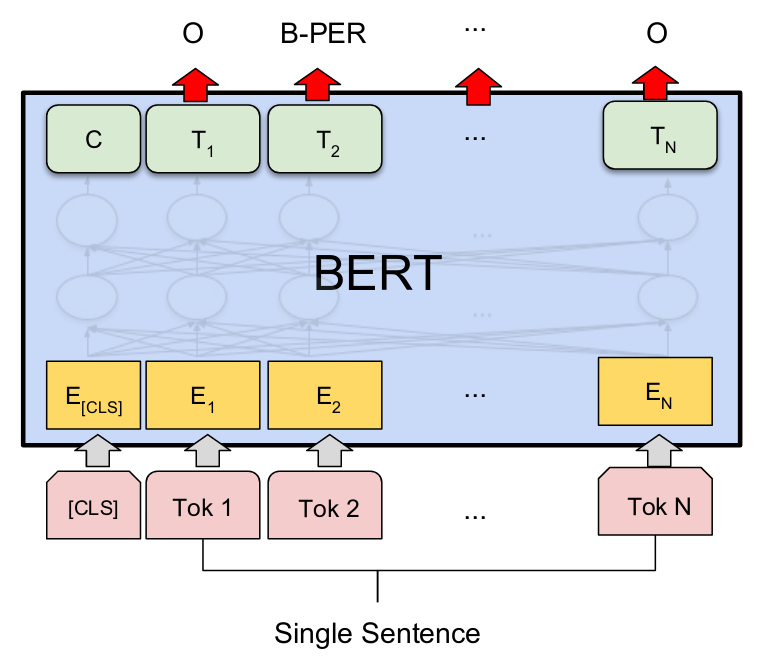
\includegraphics[width=\textwidth]{figures/bert_ner.png}
        \caption*{Single sentence tagging}
    \end{minipage}
    \caption{Two of the four single sentence tasks presented in the BERT publication~\cite[Figure 3]{devlin2018}.}
    \label{fig:bert_classification}
\end{figure}

Let $A = A_1, A_2, \cdots, A_n$ denote the layer which is depicted below $C, T_1, \cdots, T_n$, and let $B = B_1, B_2, \cdots, B_n$ denote the layer below $A$.
Let $s$ denote the number of tokens for some input sentence.
By default the max sequence length for the model is set to 128.
For each sentence the sequence length is padded to this max sequence length.
When predicting a `class label' $C$ will only be based on $A_1$ which is based on $B_1, B_2, \cdots, B_s$.
$A_2, A_3, \cdots, A_n$ are not used.
When predicting entities only $A_2, A_3, \cdots, A_s$ are used.
It seems that a joint model is possible by providing the model with a combination of these two.
Consider the NER as a base model and suppose we add some input to $C$.
Now when predicting $C$ the model is expected to learn to look at input from $A$.
For this it can use entity information from $A_2, A_3, \cdots, A_s$.
To also learn non-trivial patterns in non-entity words in the sentence it can use $A_2, A_3, \cdots, A_n$.
Typically sentences are much shorter than 128 tokens so enough space should be available in $A_2, A_3, \cdots, A_n$.
To allow for more space the max sequence length can be increased, this will increase training and inference time.

% how done
To do this the input for the model has been changed from: \\

\noindent \verb|text: ['how', 'do', 'i', 'disable', 'the', 'spam', 'filter', 'in', 'gmail', '?']|\\
\verb|true: ['O', 'O', 'O', 'O', 'O', 'O', 'O', 'O', 'B-WebService', 'O']|\\

to\\

\noindent \verb|text: ['INTENT', 'how', 'do', 'i', 'disable', 'the', 'spam', 'filter', 'in',|\\
\hspace*{12cm} \verb|'gmail', '?']|\\
\verb|true: ['FilterSpam', 'O', 'O', 'O', 'O', 'O', 'O', 'O', 'O', 'B-WebService', 'O']|\\

where `text' is passed to $C, T_1, \cdots, T_s$ and `true' to $E_{[CLS]}, E_1, \cdots, E_n$ during training.
% In the default BERT model $[CLS]$ is passed to denote that the model is used for classification.
The BERT tokenizer splits words which are not listed in the vocabulary corresponding to a pre-trained model.
INTENT is capitalized to force it to be out-of-vocabulary, it is converted by BERT to [UNK].
The goal of this is to avoid overriding the default interpretation BERT has for `intent' (or any other uncased token we choose).

% loss function
The NER loss function can be applied to the joint training without change.
This is counterintuitive because input examples have one position for the class $C$ and $s$ positions for the entities $T_1, T_2, \cdots, T_s$.
Typically sentences have around 10 tokens after tokenization.
So, the loss is based on around one intent position and ten entities.
This means that the model will learn entity recognition much quicker than intent classification.
For situations where the model is able to learn the entities quickly this is not expected to affect the performance of the intent classification significantly.
% explain more
It is expected that the only significant difference of this change is in the difficulty of the loss function.
% explain morec
